%%%%%%%%%%%%%%%%
%% Dispersion %%
%%%%%%%%%%%%%%%%
\section{Swarm Dispersion}
\subsection{Description}
This section discusses the process of evolving a swarm behavior for agent dispersion.  Physical dispersion is a fundamental swarm behavior that has many applications including establishing perimeters and performing searches.  Additionally, dispersion serves as a basis for more complex swarm behaviors as it provides a flexible method of controlling the physical configurations of a swarm without the need to exert control over each individual agent.

The goal of a dispersion algorithm is for a swarm is to achieve a physical configuration that satisfies one or more constraints, such as average neighbor distance, nearest-neighbor distances, or neighborhood densities.  Since both an agent's physical dynamics and the dispersion criteria may not be static, the physical configurations achieved by a dispersion algorithm can be either static or dynamic in nature.

%% Dispersion->Implementation
\subsection{Implementation}

For this work, a swarm of agents is deployed in a bounded environment.  In general, the initial physical configuration of the swarm is arbitrary, so a random distribution in a bounded subregion is used (see \refSection{Dispersion}).  The goal of the swarm is to expand and/or contract to achieve a specific density, specified in terms of distances between individual agents.  More formally, an agent has satisfied the dispersion criteria if all of their neighbors are at least $d_{min}$ units away, but not more than $d_{max}$, where $d_{min} < d_{max}$.  Thus in this case, a swarm achieves a successful dispersion when all agents meet the defined minimum and maximum neighbor distance criteria.

\begin{figure}[ht]
  \centering
  \includegraphics[scale=1]{DispersionSensor}
  \caption[Dispersion criteria for a single agent.]{For an agent to satisfy the dispersion criteria, all of their neighbors are at least $d_{min}$ units away, but not more than $d_{max}$, where $d_{min} < d_{max}$.}
  \label{fig:DispersionSensor}
\end{figure}

The environment for the simulation is a bounded grid-based environment.  The agents possess limited mobility and sensing capabilities.  Each agent can move in any of the four cardinal directions at a uniform speed.  Additionally, an agent is also capable of moving in a random cardinal direction or not moving at all.  The agent behaviors related to movement are \emph{move-up}, \emph{move-down}, \emph{move-left}, \emph{move-right}, \emph{move-random}, and \emph{move-none}.

%Each agent is only capable of sensing the presence of agents in their Conway neighborhood.\footnote{A Conway Neighborhood is defined as the set of squares adjacent to a given square either vertically, horizontally or diagonally.}  A neighbor sensor returns a boolean value indicating when the neighbor conditions are satisfied (true) or not satisfied (false) for a given region around the agent.  

Each agent has the ability to sense the presence of agents in its near vicinity.  The neighbor sensors are defined for the four regions around the agent (\refFigure{DispersionSensor}): above, below, left, and right.  Hence, the agent sensors available  are \emph{neighbor-above}, \emph{neighbor-below}, \emph{neighbor-left}, and \emph{neighbor-right}.  Encoded in each sensor is the information related to the dispersion criteria, \ie{} $d_{min}$ and $d_{max}$.  Each sensor returns \true{} only when there are agents in the region that are violating the dispersion criteria of the sensing agent.  Thus, the goal for each individual agent is to find a state where all of their sensors report \false{}.

The raw fitness of a solution is measured by the total number of agents violating the dispersion criteria with respect to another agent.  For example, if four agents are arranged in a square, the fitness score would be 12 because each agent is too close to the other three agents, thus violating the dispersion criteria for those three agents.  A worst-case scenario is where every agent is violating the dispersion criteria of every other agent.  If $n$ is the total number of agents, this scenario establishes a maximum error, $MAX\_ERROR = n*(n-1)$.  So, for the scenario examined here with 100 agents, $MAX\_ERROR = 100*99 = 9900$.  $MAX\_ERROR$ is then used to normalize the fitness score of each solution.  Since the fitness function is also an error function, the goal of this scenario is to minimize the error to 0.

The evolved solutions are scored using scenarios with randomized initial agent positions.  \refTable{DispersionParameters} shows the parameters used for evolving a swarm algorithm to address the dispersion problem.  All randomized operations (\ie{} solution generation, mutations, \ldots) use a random number generator with a uniform distribution.  Randomly generated solutions have exactly one state and one transition.  All transitions are generated by randomly assigning a start state and a next-state from the solution's set of states.  The sensor condition and action associated with the transition are then randomly selected from the solutions's set of sensor conditions and actions.

Each of the five mutations are applied to eight solutions (the best 6 plus two selected from random) per generation.  Mutations are applied to a copy of the selected solution, the copy is evaluated using \SWEEP{}, and is then rolled back into the main population.  Thus, after all mutations are complete, the effective population size will be 72 (the original 32 plus 40 mutated).  Additionally, a single randomly generated solution is introduced into the population at each generation.

Each solution is evaluated using \SWEEP{}.  Fitness data from each solution is collected from \SWEEP over 5 different trials.  The data from all the trials is then combined to give an accumulated set of raw fitness data.

\begin{table}[ht]
  \small
  \centering
  \begin{tabular}{|lc|}
    \hline
    \multicolumn{2}{|c|}{\em{Parameters}} \\
    Objective & Dispersion \\
    Max. Generations & 500 \\
    Population Size & 32 \\
    Number of Trials & 5 \\
    \hline
    \hline
    \multicolumn{2}{|c|}{\em{Mutations}} \\
    Change-Sensor-Value & top 6 + 2 random \\
    Change-Action-Value & top 6 + 2 random \\
    Change-Next-State & top 6 + 2 random \\
    Add-State & top 6 + 2 random \\
    Add-Transition & top 6 + 2 random \\
    \hline
    \hline
    \multicolumn{2}{|c|}{\em{Actions}} \\
    move-up     & move-down  \\
    move-left   & move-right \\
    move-random & move-none  \\
    \hline
    \multicolumn{2}{|c|}{\em{Sensors}} \\
    neighbor-above & neighbor-below \\
    neighbor-left  & neighbor-right \\
    \hline
    \hline
    \multicolumn{2}{|c|}{\em{Simulation}} \\
    Number of Agents & 100 \\
    Environment & $50 \times 50$ grid \\
    Maximum time & 400 \\
    \hline 
  \end{tabular}
  \caption{Parameters for evolving dispersion}
  \label{tab:DispersionParameters}
\end{table}

\subsection{Results}

In all of the evolutionary runs, a general fitness trend is observed.  Initial generations produce very poor results, with most candidate solutions scoring near the very bottom of the scale.  Gradual progress is then made for a short period, then a dramatic jump in fitness occurs.  The process of spiking and stabilizing continues one or more times until a solution with the target fitness value is evolved.  The characteristics of the fitness over time is not typical of traditional evolutionary computing fitness trends, which have a steady improvement as generations progress~\cite{back:ec1}.  One large contributing factor is the granularity of the fitness function.  Traditional fitness functions produce real-valued fitness measures, thus small improvements introduced through mutation manifest themselves as slight improvements in fitness.  In this case, since the fitness function is integer based and thus discrete valued, the slight improvements introduced through mutation may be overlooked.  Thus, the fitness function is coarse-grained and does not provide enough information to effectively drive the selective pressure of evolution.  Fortunately though in this case, the fitness function as defined does produce enough information to drive evolution towards an acceptable solution.

A typical evolutionary run for dispersion is shown in \refFigure{DispersionResults-1}.  In the first few generations, fast progress is made as the initially random solutions are modified through mutation.  Then a period of no progress occurs, lasting for about 20 generations.  However, after generation 29, there is a sharp decline in both the best and average scores, indicating that one of the evolutionary operators made a change in one of the solutions that resulted in an almost correct solution to the dispersion problem.  Yet another period of little progress occurs, this time lasting until a fully-functioning dispersion algorithm is found in generation 111.  The resulting evolved state machine for dispersion is shown in \refTable{DispersionAlgorithm}. 

\begin{table}[ht]
\centering
\caption{Evolved dispersion state machine}
\footnotesize
\begin{tabular}{|c|c|l|p{6ex}|}
  \hline
  State & Condition & Action & Next State \\
  \hline
  \begin{slide}{Dispersion}
  \begin{itemize}
  \item Swarm Goal: achieve a density level
  \item Agent Goal: 
    \begin{itemize}
    \item neighbor at least $d_{min}$ units away
    \item neighbor not more than $d_{max}$ units away
    \end{itemize}
  \end{itemize}
  \centering
  \includegraphics[scale=.18]{DispersionSensor}
\end{slide}

%%%%%
%%%%%

\begin{slide}{Dispersion}
  \begin{itemize}
  \item Fitness: Number of agents violating dispersion criteria
  \end{itemize}
  \centering
  \begin{tabular}{l|l}
    \textbf{Actions} & \textbf{Sensors} \\
    \hline
    move-up    & neighbor-above \\
    move-down  & neighbor-below \\
    move-left  & neighbor-left  \\
    move-right & neighbor-right \\
  \end{tabular}
  \begin{itemize}
  \item Population: 32
  \item Mutations: all top 6 + 2 random
  \item \SWEEP: 100 agents, $50\times50$ grid
  \item $d_{min} = 2$, $d_{max} = 4, range = 6$
  \end{itemize}
\end{slide}

%%%%%
%%%%%

\begin{slide}{Dispersion}
  \centering
  \includegraphics[scale=.5]{DispersionRun1}
\end{slide}

\end{tabular}
\label{tab:DispersionAlgorithm}
\end{table}

% Also need to show average and standard deviation
\begin{figure}[ht]
	\centering
	\includegraphics[scale=.75]{Figures/DispersionRun1.pdf}
\caption{Best and average fitness scores resulting from evolving a dispersion algorithm.}
\label{fig:DispersionResults-1}
\end{figure} 

% Also need to show average and standard deviation
%\begin{figure}[ht]
%	\centering
%	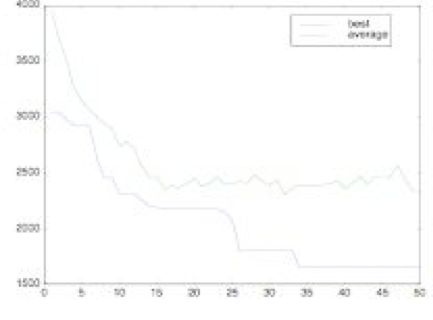
\includegraphics[scale=.25]{Figures/DispersionRun2.pdf}
%	\caption{Best and average fitness scores from evolving a dynamic equillibrium dispersion algorithm.}
%	\label{fig:DispersionResults-2}
%\end{figure} 

\clearpage
